\section{Aggiungi un nuovo profilo} {
    Dalla pagina iniziale Home è possibile accedere alla pagina ``\textbf{Add}'' cliccando sulla barra di navigazione il pulsante con tale scritta.
    \aCapo
    In questa pagina, utilizzando la barra di ricerca, è possibile cercare un profilo che non si segue, scrivendo il suo username e cliccando poi il bottone di ``\textbf{Search}''. 
    
    \begin{figure}[H]
        
\includegraphics[width=12cm]{sezioni/images/add.png}
        \centering
        \caption{Cercare un nuovo profilo social}
    \end{figure}
    
    Successivamente comparirà il profilo che si è cercato con le seguenti informazioni:
    \begin{itemize}
        \item Username del profilo;
        \item Il suo numero di followers (persone che lo seguono);
        \item Il bottone ``\textbf{Segui}'' che una volta cliccato permetterà di aggiungere il profilo a quelli seguiti.
    \end{itemize}

    \begin{figure}[H]
        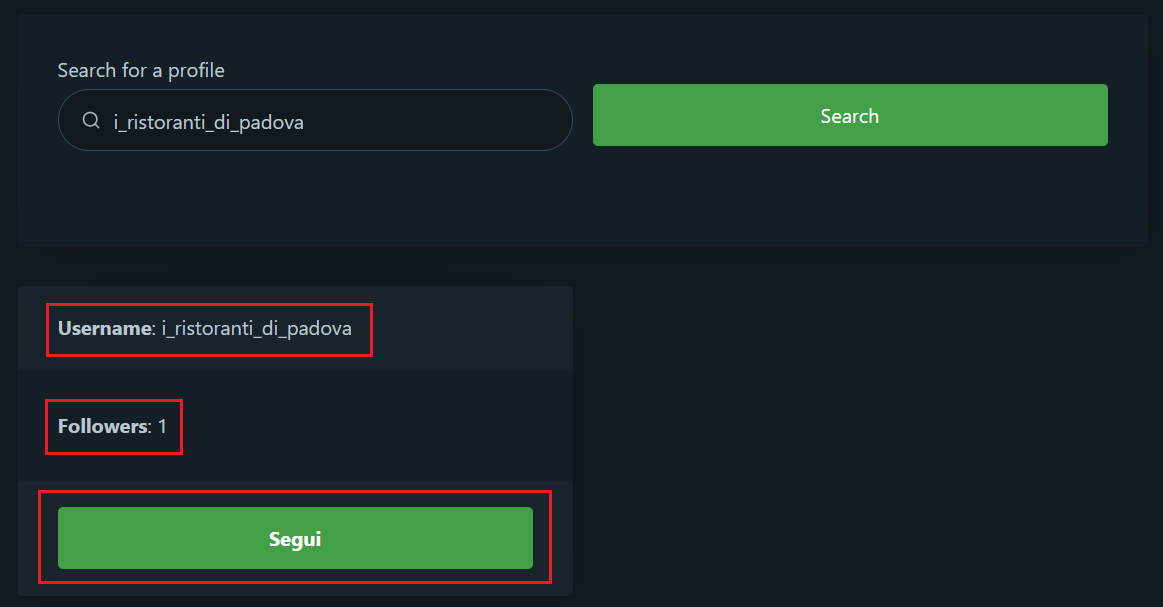
\includegraphics[width=12cm]{sezioni/images/risultato-add.png}
        \centering
        \caption{Risultato del profilo social cercato}
    \end{figure}

    \subsection{Errore username} {
    \begin{enumerate}
        \item Se il campo di compilazione rimane vuoto, il sistema rileverà un errore, mostrando il seguente messaggio: 
        \begin{figure}[H]
            
\includegraphics[width=12cm]{sezioni/images/err1-add.png}
            \centering
            \caption{Errore - non è stato scritto nessuno username}
        \end{figure}
        \item Se invece l'username non è scritto correttamente, il sistema non riuscirà a trovare il profilo. Infatti la ricerca avviene puramente sul contenuto scritto all'interno della barra di ricerca.
        \begin{figure}[H]
            
\includegraphics[width=12cm]{sezioni/images/err2-add.png}
            \centering
            \caption{Errore - l'username cercato non esiste}
        \end{figure}
        \item Se invece l'username cercato è già tra i profili seguiti, comparirà un errore di questo tipo:
        \begin{figure}[H]
            
\includegraphics[width=12cm]{sezioni/images/err3-add.png}
            \centering
            \caption{Errore - l'username cercato è già seguito}
        \end{figure}
    \end{enumerate}
    }
}
